\documentclass[a4 paper, 10pt]{article}
\usepackage[utf8]{inputenc}

\usepackage{natbib}
\usepackage{graphicx}
\usepackage[a4paper, total={6in, 8in}]{geometry}

\title{IF679 - Informática e Sociedade}
\author{Thiago Henrique}
\date{Outubro 2019}

\begin{document}

\maketitle

\section{Introdução}
A disciplina de Informática e Sociedade é ofertada aos alunos de Ciência da Computação (Profª Carina Frota Alves) e Engenharia da Computação (Profª Verônica Teichrieb) no 3º período, e tem como objetivo de ensinar conceitos básicos de sociologia, além de ser a cadeira "responsável por relacionar e refletir sobre o relacionamento da sociedade num âmbito tecnológico." \cite{sitepet}

\section{Relevância}
No mundo atual, onde a tecnologia tem um profundo impacto em toda a sociedade nos mais diversos setores, é de extrema importância refletir e analisar esse impacto, seja positivo e negativo, afim de criar profissionais conscientes do impacto do seu trabalho na sociedade, e que ele possa contribuir para o desenvolvimento social da sua localidade.

\begin{figure}[h!]
\centering
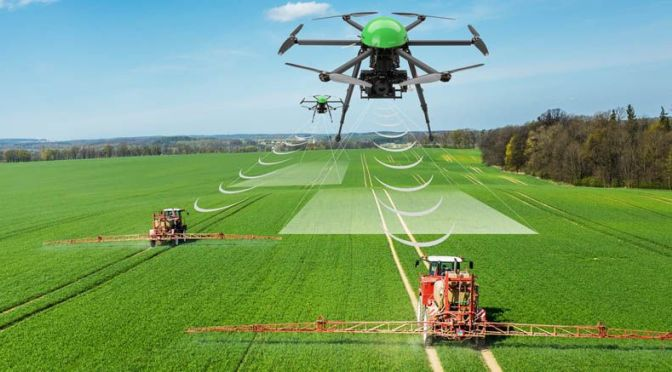
\includegraphics[scale=0.4]{drone-agricola.jpg}
\caption{Drone Agrícula \cite{drone}}
\label{fig:drone-agricola.jpg}
\end{figure}

\section{Relação com as outras disciplinas}
A cadeira de Informática e Sociedade não possui pré-requisito e também não é pré-requisito de nenhuma outra disciplina.\cite{perfil}  Porém, sendo uma disciplina obrigatória, ela é de fundamental importância para a conclusão dos cursos de Ciência da Computação e Engenharia da Computação.

\bibliographystyle{plain}
\bibliography{References}
\end{document}